\documentclass[11pt,article,oneside]{memoir}
\usepackage{org-preamble-xelatex}
\input{vc}


\usepackage{graphicx}
% We will generate all images so they have a width \maxwidth. This means
% that they will get their normal width if they fit onto the page, but
% are scaled down if they would overflow the margins.
\makeatletter
\def\maxwidth{\ifdim\Gin@nat@width>\linewidth\linewidth
\else\Gin@nat@width\fi}
\makeatother
\let\Oldincludegraphics\includegraphics
\renewcommand{\includegraphics}[1]{\Oldincludegraphics[width=\maxwidth]{#1}}

\title{\bigskip \bigskip Introduction}
 
\author{\bigskip\Large Jason A. Heppler}

\begin{document}  

\setsansfont[Mapping=tex-text, BoldFont={* Bold SemiCondensed}, ItalicFont={* Semibold SemiCondensed Italic}]{Myriad Pro}
\setmonofont[Mapping=tex-text,Scale=MatchLowercase]{Consolas}
\setromanfont[Mapping=tex-text,Numbers=OldStyle]{Minion Pro}


\setkeys{Gin}{width=1\textwidth}  
\setromanfont[Mapping=tex-text,Numbers=OldStyle]{Minion Pro} 
\setsansfont[Mapping=tex-text]{Minion Pro} 
\setmonofont[Mapping=tex-text,Scale=0.8]{Consolas}
\chapterstyle{article-4} 
\pagestyle{kjh}

\published{Draft only. Please do not cite without permission.}

\maketitle


\begin{quote}
The underlying principle of conservation has been described as the
application of common sense to common problems for the common good. If
the description is correct, then conservation is the great fundamental
basis for national efficiency. In this stage of the world's history to
be fearless, to be just, and to be efficient are the three great
requirements of national life. National efficiency is the result of
natural resources well handled, of freedom of opportunity for every man,
and of the inherent capacity, trained ability, knowledge and will,
collectively and individually to use that opportunity."

-- President Theodore Roosevelt (1909)
\end{quote}

\begin{quote}
In time and with water, everything changes.

-- Leonardo da Vinci
\end{quote}

Looking back on the four decades since William Hewlett and Richard
Packard founded their high technology company in a Palo Alto garage, the
\emph{San Jose Mercury}, the city's oldest newspaper, through a series
of articles surveyed ten causes of Silicon Valley's success. One of
those causes was environmental: water. Beginning in 1965, water from the
Sacramento-San Joaquin River Delta flowed forty-four miles through the
South Bay Aqueduct, bringing \{number\} gallons of water to
\{location\}. Sig Sanchez, who was serving as the director of the Santa
Clara Valley Water District in the 1990s, recalled the project's
importance to Silicon Valley. ``It was our first import project, and it
was essential to the growth we were anticipating,'' he remarked. ``The
valley would have grown, but not at the rate it has, because we would
not have been able to accommodate the Silicon Valley.''\footnote{``Water
  made orchards, silicon chip industry sprout faster,'' \emph{San Jose
  Mercury}, December 22, 1999.} Water and economic growth went hand in
hand.

Three large water projects would eventually bring a consistent source of
fresh water into Santa Clara Valley. Twenty years after the South Bay
Aqueduct, the San Felipe water system would be constructed through
Pacheco Pass to move water out of the San Joaquin Valley. Additionally,
the Valley consumed water from the Hetch Hetchy system, which today
supplies about half the water used throughout the Bay. Additional water
conservation projects, including dams, reservoirs, percolation ponds,
canals, and runoff capture, together helped provide the Valley with its
water needs. James Lenihan, who served on the water conservation board
in the 1960s and later served on the board for the Santa Clara Valley
Water District, credited water project success on the absence of an
environmental movement. ``With the environmental movement, we would
never have been able to do now what we did then,'' he said. ``We were
able to get it in place before the movement came along to say no more
reservoirs, no pipelines, no aqueducts.''\footnote{``Water made
  orchards, silicon chip industry sprout faster,'' \emph{San Jose
  Mercury}, December 22, 1999.}

Unrestricted urban growth and economic development characterized much of
Santa Clara Valley in the latter half of the twentieth century, but
little told is the story of the environmental consequences of Silicon
Valley and those who attempted to shape the conversation about the
region's ecological future.(On the rise of the modern environmental
movement, see: Hays 1987, 13--39; H. Rothman 2000, 131--159; Steinberg
2002, 239--261; Opie 1998, 404--433.) California voters became
increasingly aware of the environmental considerations urban growth and
industrial development had for their region, leading by 1973 to voters
rejecting new large-scale water projects. Furthermore, environmental
groups such as the Friends of the Earth, the Sierra Club, and Silicon
Valley Toxics Coalition criticized high technology firms and city
leaders for their ignorance on environmental change. The costs of
environmental negligence became most obvious in the 1980s, when cancer
clusters emerged in San Jose. The source of the cancer clusters was
traced back to semiconductor manufacturers, whose toxic waste storage
tanks were discovered leaking and contaminating underground aquifers.
The water in the aquifers are still unusable today.\{source\}

The story told here stands at the intersections of postindustrial
society, environmental history, and the spatial politics of
suburbanization and economic development. City leaders, residents,
laborers, migrant workers, and others all experienced rapid urban change
after World War II and responded in various ways to these changes. One
consequence of these changes is the enormous demands made upon water
resources in the Far West.

Silicon Valley has only just begun to attract attention of historians.
Margaret O'Mara and John Findley have written the best accounts of
Silicon Valley and its place in urban processes. But their stories focus
on the institutional and cultural construction of Silicon Valley.

\begin{figure}[htbp]
\centering
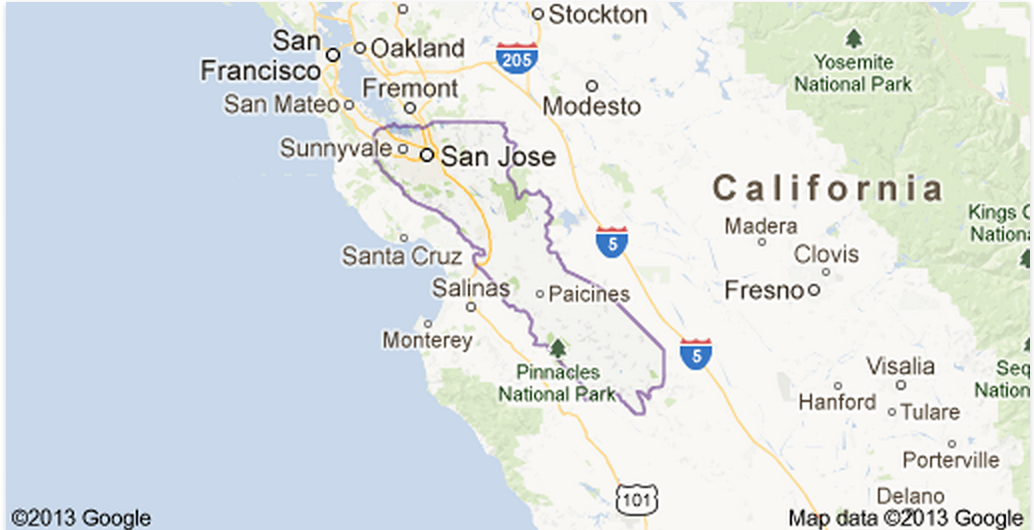
\includegraphics{/Users/jheppler/Projects/Dissertation/figures/sv.png}
\caption{Silicon Valley. The Santa Clara Valley lies between the Santa
Cruz Mountains on the west and the Diablo Range to the east, largely
encompassing the municipalities of San Jose, Mountain View, Sunnyvale,
Palo Alto, Menlo Park, and Redwood City. Between 1945 and 2000, San Jose
became the largest city in the Bay Area and ranked the near the top of
population growth in the nation.}
\end{figure}

Metropolitan growth, annexations, and incorporations were so rapid that
Robert Self called the process a ``land rush.''(Self 2003, 20.)

The study approaches political history at the local level. City leaders,
activists, and residents shaped the implementation and interpretation of
policies \ldots{}

In examining the human and environmental costs of water, electronics,
outdoor recreation, urban development, and wilderness areas, this study
evaluates the costs of these programs. Although this study is tightly
focused on a specific region, it has greater bearing on understanding
the inherent tension between local and national politics. In the Santa
Clara Valley, the development of new landscapes, resulting from various
perceptions of the region as farmland, electronics manufacturer, urban
oasis, and tourist destination shaped the use of water in the valley.

Water and technology are icons in California. The battle over the Hetch
Hetchy reservoir and the growth of environmentalism calls to mind the
importance of water and its battles in the Far West, while the
electronics industry has located its origin myth in the former orchard
fields surrounding Stanford University. These two icons share the
California landscape in ways not yet examined by historians. Although
considered separate landscapes, they are entangled in ways not
previously understood. Water and the Santa Clara Valley share what
Richard White has called a hybrid landscape. Neither rural or urban,
hybrid landscapes are complex creations of natural and cultural systems
that shape a place.(White 2004. In surveying the trends in environmental
history, Richard White reviewed the works of several environmental
historians including Josephy Taylor, Mark Fiege, Nancy Langston, and
William DeBuys, who reject any hard division between culture and
natural. Instead, they examine how forces shape and inform landscapes.
Kenneth Olwig has argued that landscape is substantive, where
``enivronment, economics, law, and culture are all important,'' and
smbolic, ``to be perceived, read, and interpreted on the ground, in
written texts, and through artistic images.'' ; Sauer 2008, 100; Olwig
1996, 645; Meinig 1979, 43--45; Basso 1996, 110.)

Water became a linchpin in contests over power conflicts: who controlled
water, who had access to water, how water should and could be used. The
valley's agricultural past required access to water to support orchard
fields. Later in the twentieth century, water became key to
semiconductor manufacturers, who used an ultra-purified water in the
process of manufacturing electronics components. Supporting urban growth
offered a third theme in contests over water, as the valley's population
exploded in the mid-twentieth century. And finally, residents new and
old made demands on water as recreation. Dam projects by the state of
California in and around the Santa Clara Valley became tied to
recreation and tourism while simultaneously supporting other water
projects for manufacturing and urban growth. As water demands rose, it
also gave growth to a modern environmental movement that challenged
suburban sprawl, industrial development, and recreation in the Bay Area
while also breathing life into environmental movements across the
nation.

\textbar{} \textbar{} Less Than 100 Acres \textbar{} More Than 100 Acres
\textbar{}
\textbar{}:----:\textbar{}:-------------------:\textbar{}:--------------------:\textbar{}
\textbar{} 1880 \textbar{} 721 \textbar{} 771 \textbar{} \textbar{} 1890
\textbar{} 1,427 \textbar{} 750 \textbar{} \textbar{} 1900 \textbar{}
3,057 \textbar{} 938 \textbar{} \textbar{} 1910 \textbar{} 3,096
\textbar{} 825 \textbar{} \textbar{} 1920 \textbar{} 4,390 \textbar{}
626 \textbar{} \textbar{} 1930 \textbar{} 5,616 \textbar{} 621
\textbar{}

Table: Number of Farms in Santa Clara County, by Size, 1880-1930.
Adapted from Lukes (1994), p.~382.

Efforts by federal regulators, city officials, business leaders, and
farmers all attempted to maximize their access to water. Beginning in
the 1930s, orchard fields in the Santa Clara Valley became national
producers of prunes, cherries, peaches, \{more\}. The growing
agribusiness presence in the Bay Area made demands on local water
resources and led federal officials and state political leaders to
pursue water and irrigation projects that would sustain farmlands. Yet
by the 1930s so much water was being pumped out of underground water
basins that Stanford geologists discovered Santa Clara Valley had sunk
four feet in just twenty years.\footnote{``Data Show Sinking of Bay
  Area,'' \emph{Los Angeles Times}, March 20, 1934, p.~1. The process of
  land sinking is known as subsidence and results from the weight of
  land compacting underground sand and gravel aquifers that have been
  drained. Subsidence would not end until 1969; by then, downtown San
  Jose had sunk ten feet and Alviso along the coastal bay had sunk
  thirteen feet.} Concerns over the Valley's access to water led to the
development of the Central Valley Project in the late 1930s.

South Bay Aqueduct and San Joaquin Valley Project, along with San
Francisco's Hetch Hetchy reservoir, supplied over half the water to the
Valley. The water projects were essential to support the growing
suburbs, high tech industries, and agriculture in the Valley.

The story here re-situates how we understand Silicon Valley by placing
the environment at the core of the story. \{EXPAND\}

Postwar prosperity encouraged widespread growth across the country. By
the 1950s a majority of American cities achieved wide growth, but what
was initially seen as a fulfillment of the American dream of
homeownership became viewed as an environmental disaster. Critics took
aim at suburban growth and environmental destruction, and nowhere was
this change more obvious than in the West. Metropolitan growth doubled
the population in the region between 1940 and 1960. Many westerners were
unsettled by population growth, and raised concerns about the
disappearance of rural landscapes being replaced by sprawl. Western
political leaders such as Oregon Governor Thomas McCall condemned what
he called ``sagebrush suburbs'' and sought limits on growth in the
state. Other anti-growth sentiments emerged in \{example\}. By the
1980s, the region was among the fastest growing in the nation.(On
environmental concerns over suburbanization see: Jackson 1985; Rome
2001.)

The urban expansion of the Bay Area and its demands for water resources
coincided with the growing environmental movement in America. Beginning
in the 1960s, environmental groups like Sierra Club became politically
active. The Wilderness Act of 1964 likewise brought greater attention to
the nation's environmental issues. By the late 1960s, the environmental
movement had become ``a mass movement organized around cleaner air and
water for all, not just in wilderness areas.''(Steinberg 2002, 240.)
Books about the environment became best sellers, notably Rachel
Carlson's \emph{Silent Spring} and Paul and Anne Ehrlich's \emph{The
Population Bomb}. Other legislative actions, including the National
Environmental Policy Act (NEPA) and the Clean Air Act and Clean Water
Act, reflected growing concerns over environmental issues.(Hays 1987,
13--39; Opie 1998, 404--433; H. Rothman 2000, 131--159; Steinberg 2002,
250--257.)

\section{Water and the West}

Historians of western America have long identified water as a central
component in the region's historical experience. Frederick Jackson
Turner \ldots{}..

Walter Prescott Webb's classic The Great Plains (193?) revised Turner's
telling of Western history and located in the Plains a different, if not
outright hostile, environment --- an experience far different from the
environment Turner's Americans experienced in the East. For Webb, water
was a defining feature of the Great Plains: he bounded the region based
on its precipitation; he recounted the region's troubles with
agriculture and water use; he maintained the importance of irrigation
projects; etc. Having no trees and scarce water, the Great Plains
settlers

\begin{quote}
Were thrown by Mother Necessity into the clutch of new circumstances.
Their plight has been stated in this way: east of the Mississippi
civilization stood on three legs--land, water, and timber; west of the
Mississippi not one but two of these legs were withdrawn,--water and
timber,--and civilization was left on one leg--land. It is small wonder
that it toppled over in temporary failure.
\end{quote}

Webb's settlers turned to underground aquifers -- their only source of
substantial water -- and developed new methods for dealing with scarce
resources: irrigation systems, new legal systems for allocating water
rights. The prairie was ``a land of survival where nature has most
stubbornly resisted the efforts of man. Nature's very stubbornness has
driven man to the innovations which he has made.'' Struggle against a
resistant environment has been told by subsequent historians. James
Malin's more ecologically sophisticated studies of the Plains tells a
similar story of settlers moving from ``forest man'' to ``grass man.''
Paul Bonnifield's The Dust Bowl provides a similar narrative of humans
overcoming the environment.

\section{Postwar Western Demographics}

The mobilization of the country in World War II dramatically altered the
nation and people's daily lives. Following a decade of economic
depression, people migrated to metropolitan areas to take new wartime
industries. The American West especially felt the impact of this
demographic shift, leading Carl Abbott to remark that launched ``the
entire West into the half-century of head-long urbanization.''(Abbott
1995, 4.) Six of the largest western metropolitan areas grew in 1940
grew by 380\% over the course of fifty years, compared to just 64\% for
the six largest in the East.(Abbott 1995, p.~xiii.) Just as populations
were migrating to metropolitan centers, the number of people living
inside city boundaries was declining. The attraction of suburban life
\{EXPAND\}

\section{The Bay Area}

The San Francisco Bay Area is among the most highly populated places in
the United States. The area is physiographically situated between the
Santa Cruz mountains to the west and the Diablo Range to the east, a
tightly compact area spanning only \{MILES\} across and \{MILES\} long.
Hydrologically, the region is fed by several rivers and aquifers
dominated by the \{FACT\}.

\begin{figure}[htbp]
\centering
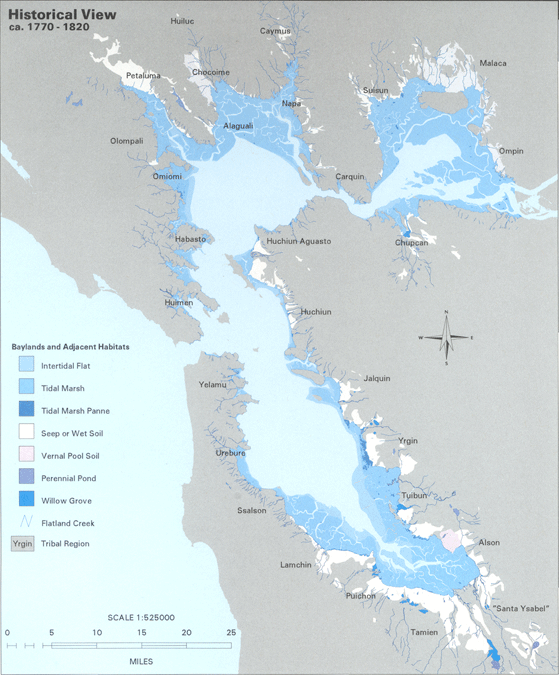
\includegraphics{/Users/jheppler/Projects/Dissertation/figures/hydrology.png}
\caption{Bay Area hydrology.}
\end{figure}

The Mediterranean climate of the Bay Area means the region receives very
little rainfall outside of the period between November and April. Around
seven percent of California land in 1951 was agricultural, and around
half of that land required consistent irrigation.(Blaney 1951) On
average, the semiarid Valley receives about 14 inches of rain
annually.\footnote{``Water made orchards, silicon chip industry sprout
  faster,'' \emph{San Jose Mercury}, December 22, 1999.}

\section{The Landscape of Conflict}

Geographer John Wright argued that ``places are best seen as shifting
stages where the exercise of power and resistance to it vie for
dominance.''

Questioning the need for water projects at all.

\begin{figure}[htbp]
\centering
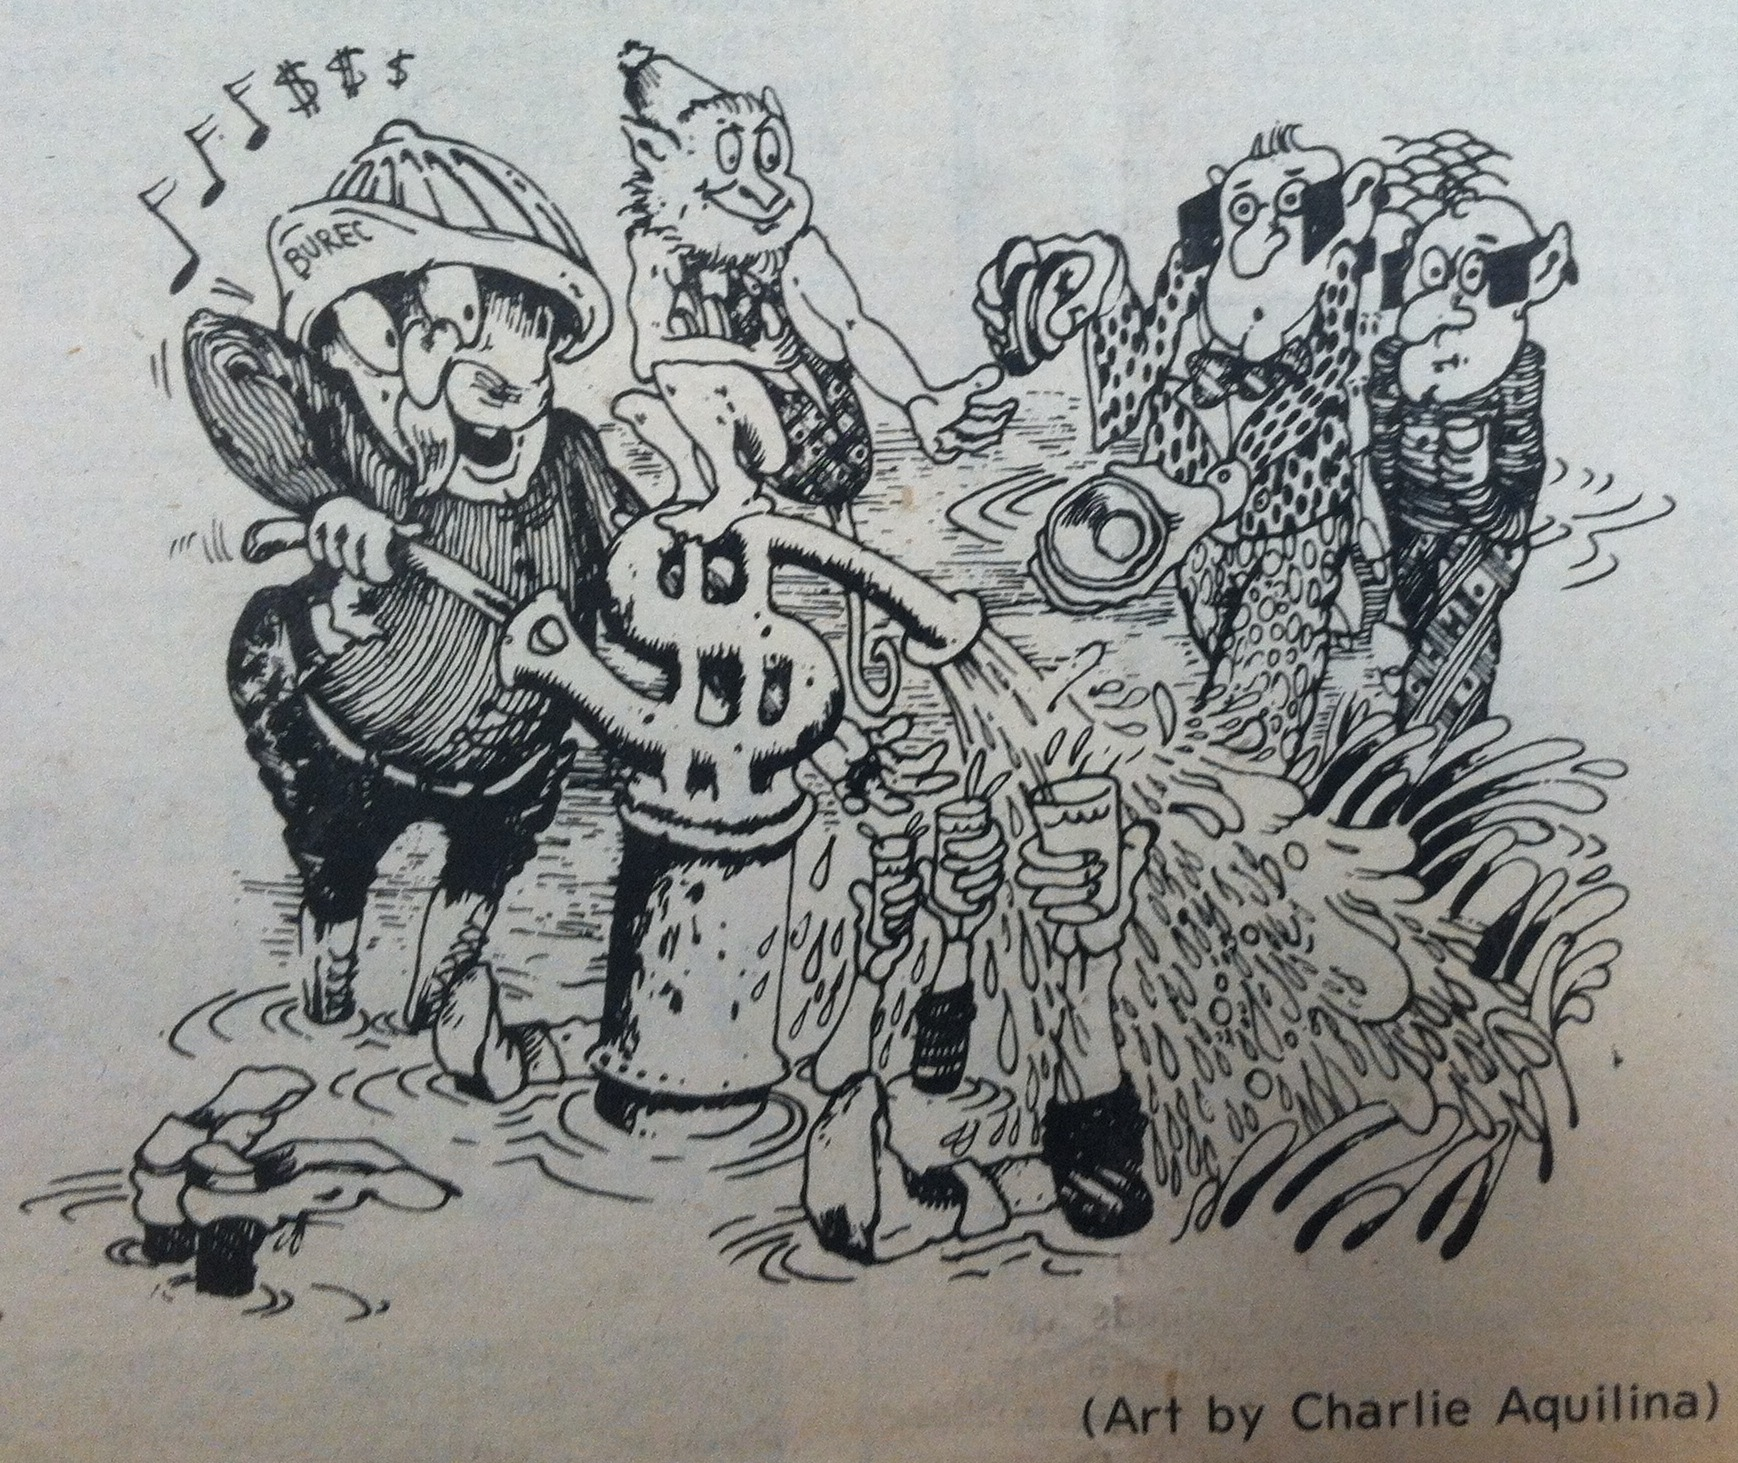
\includegraphics{/Users/jheppler/Projects/Dissertation/figures/money_waste.jpg}
\caption{Water waste}
\end{figure}

\section{Organization}

The dissertation is organized chronologically and thematically. Each
chapter is roughly chronological to one another, but thematic in their
narrative to explore the various processes and contests at work in the
Valley. The themes are organized around irrigation, manufacturing,
tourism, and urban growth.

\textbf{Chapter 1: The Western Water Landscape}

The water landscape

The urban landscape

The agricultural landscape

The industrial landscape

\textbf{Chapter 2: The Valley of Heart's Delight}

agriculture

\textbf{Chapter 3: ``Carved from a Forest of Fruit Trees'': Urban Growth
and Water Resources}

urban

Joe Ruscigno, a lifetime farmer and resident of the Valley, had started
a new occupation in 1952. ``Guess I've pulled out 150 acres of trees
since the first of the year,'' he told the San Francisco Chronicle.
Ruscigno lamented the uprooting of the prune trees to the bulldozer he
now sat upon, but ``what can you do? . . . The subdivisions were coming
in all around us and when they made a good offer I sold out.''\footnote{``Santa
  Clara County -- Scene of the Big Boom,'' \emph{San Francisco
  Chroncile}, May 11, 1952.} The Valley's suburbanization led to similar
experiences as those by Ruscigno.

Chapter 3 builds chronologically from the previous chapter and extends
the story into the World War II and postwar years.

\textbf{Chapter 4: How Clean is Clean?}

Industry

\textbf{Chapter 5: Leisure, Recreation, and Water}

recreation

Just as urban and business resources were making greater demands on the
Valley's water resources, a shift in thought about the utility of water
resources became centered on the experiential value of outdoor
recreational tourism. Recreation presented an opportunity to use water
that could continue to fuel monetary values into the Valley.\footnote{Shaffer
  (2001) and Louter (2006). For a similar history of the national
  forests and the ways in which the American public interacted with them
  through activities such as skiing, hiking, and camping see Sutter
  (2002), Wolf (2008), Childers (2010). Clawson and Held (1957), p.~341;
  H. K. Rothman (1998), pp.~23-25.}

\subsubsection{NOTES}

\begin{enumerate}[(1)]
\setcounter{enumi}{146}
\item
  ``massive military expenditures have spurred a major spatial shift in
  manufacturing production to the so-called defense perimeter. In this
  manner, the federal government, by means of its military budget and
  locational preferences, has promoted uneven regional development.''
\item
  ``At the center of these processes of economic structuring and spatial
  shifts is the information sector, which includes both information
  technologies (the hardware part) and the use of advanced information
  systems (the software part). The spatial consequences of these
  information technologies and systems deserve more attention from
  historians than they have received. Introduction of these new
  technologies in the manufacturing and service sectors, for example,
  directly affects where businesses choose to locate -- since it reduces
  the need for spatial proximity.''
\item
  Sees Orange County as a leader in these processes -- economic
  restructuring, militarization of production, spatial transformation,
  information technologies and systems, internationalization of a
  regional economy. --- Olin article (above)
\end{enumerate}

Santa Clara County came to dominate cultural and commercial influence in
the United States, becoming what Carl Abbott called the ``new centers
for American life.''

Abbott, Carl. 1995. \emph{Metropolitan Frontier: Cities in the Modern
American West}. Tucson: University of Arizona Press.

Basso, Keith H. 1996. \emph{Wisdom Sits in Places: Landscape and
Language Among the Western Apache}. Albuquerque: University of New
Mexico Press.

Blaney, Harry F. 1951. ``Use of Water by Irrigated Crops in
California.'' \emph{Journal of the American Water Works Association} 43
(3) (mar): 189--200.
\href{http://www.jstor.org/stable/41235720}{http://www.jstor.org/stable/41235720}.

Childers, Michael. 2010. ``Fire on the Mountain: Growth and Conflict in
Colorado Ski Country.'' University of Nevada, Las Vegas.

Clawson, Marion, and Burnell Held. 1957. \emph{The Federal Lands: Their
Use and Management}. Baltimore: Resources for the Future, Inc.

Hays, Samuel P. 1987. \emph{Beauty, Health, and Permanence:
Environmental Politics in the United States, 1955-1985}. Cambridge:
Cambridge University Press.

Jackson, Kenneth T. 1985. \emph{Crabgrass Frontier: The Suburbanization
of the United States}. New York: Oxford University Press.

Louter, David. 2006. \emph{Windshield Wilderness: Cars, Roads, and
Nature in Washington's National Parks}. Seattle: University of
Washington Press.

Lukes, Timothy J. 1994. ``Progressivism Off-Broadway: Reform Politics in
San Jose, California, 1880-1920.'' \emph{Southern California Quarterly}
76 (4) (winter): 377--400.

Meinig, Donald. 1979. ``The Beholding Eye: Ten Versions of the Same
Scene.'' In \emph{The Interpretation of Ordinary Landscapes The
Interpretation of Ordinary Landscapes}, ed. Donald Meining and Donald
Meinig, 43--45. New York: Oxford University Press.

Olwig, Kenneth R. 1996. ``Recovering the Substantive Nature of
Landscape.'' \emph{Annals of the Association of American Geographers}
(dec): 645.

Opie, John. 1998. \emph{Nature's Nation: An Environmental History of the
United States}. Fort Worth: Harcourt Brace College Publishers.

Rome, Adam. 2001. \emph{Bulldozer in the Countryside: Suburban Sprawl
and the Rise of American Environmentalism}. New York: Cambridge
University Press.

Rothman, Hal. 2000. \emph{Saving the Planet: The American Response to
the Environment in the Twentieth Century}. Chicago: Ivan R. Dee.

Rothman, Hal K. 1998. \emph{Devil's Bargains: Tourism in the Twentieth
Century American West}. Lawrence: University Press of Kansas.

Sauer, Carl. 2008. ``The Morphology of Landscape.'' In \emph{The
Cultural Geography Reader The Cultural Geography Reader}, ed. Timothy S.
Oakes and Patricia L. Price, 100. New York: Routledge.

Self, Robert O. 2003. \emph{American Babylon: Race and the Struggle for
Postwar Oakland}. Princeton: Princeton University Press.

Shaffer, Marguerite S. 2001. \emph{See America First: Tourism and
National Identity, 1880-1940}. Washington, D.C.: Smithsonian Institution
Press.

Steinberg, Ted. 2002. \emph{Down to Earth: Nature's Role in American
History}. New York: Oxford University Press.

Sutter, Paul S. 2002. \emph{Driven Wild: How the Fight Against
Automobiles Launched the Modern Wilderness Movement}. Seattle:
University of Washington Press.

White, Richard. 2004. ``From Wilderness to Hybrid Landscapes: The
Cultural Turn in Environmental History.'' \emph{The Historian} 66 (sep):
562--664.

Wolf, Tom. 2008. \emph{Arthur Carhart: Wilderness Prophet}. Boulder:
University of Colorado.


\end{document}
